The runtime view is explained with the help of sequence diagrams, which shows the interaction between the components during runtime in a time flow depicting the order of which function takes place after another. The function names are same as the interface in order to help to relate the component, their interaction and their behavior during runtime. The interfaces are very descriptively explained in the component  diagram and they function the same here.The sequence diagram of the three major services of TrackMe are shown which comprises the entire functioning of TrackMe and integrates to make the complete application.\newline
Here are the three sequence diagrams which briefly summarizes the runtime of the application.
\begin{figure}[H]
	\begin{center}
		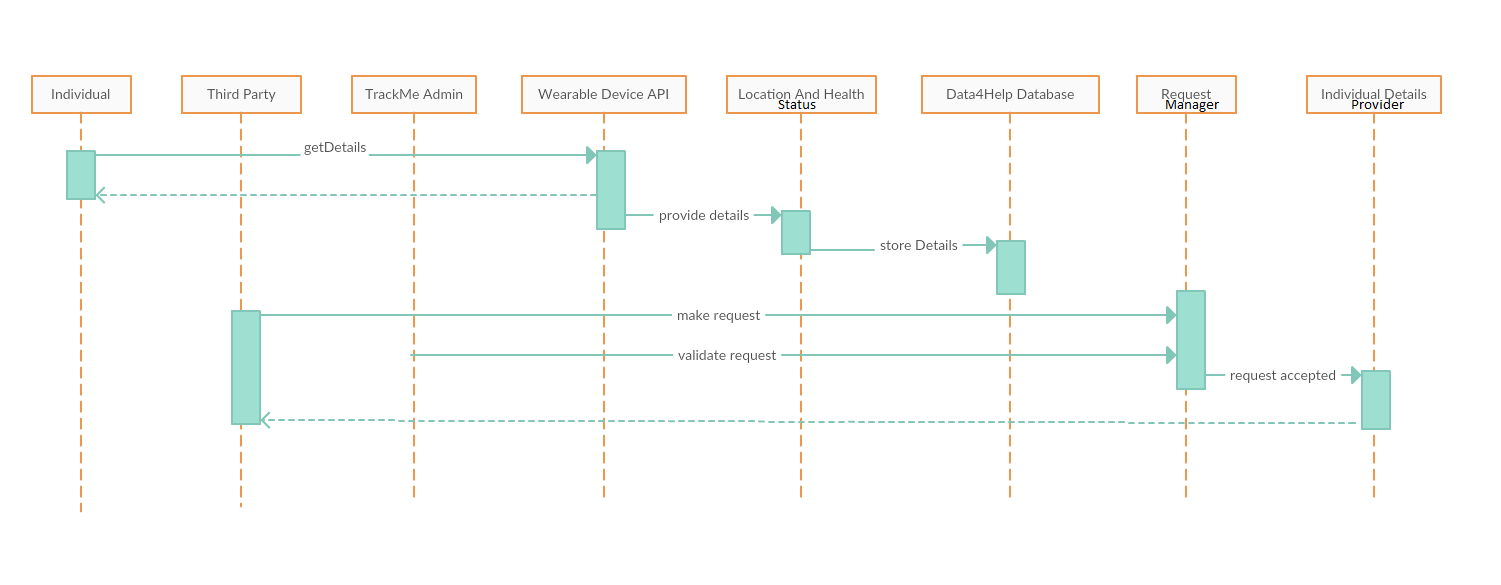
\includegraphics[width=\textwidth]{./DD_Diagrams/RuntimeData4Help.png}
      \caption{Sequence Diagram depicting runtime of Data4Help Service}
        \label{TrackMe_r1}
	\end{center}
\end{figure}
\begin{figure}[H]
	\begin{center}
		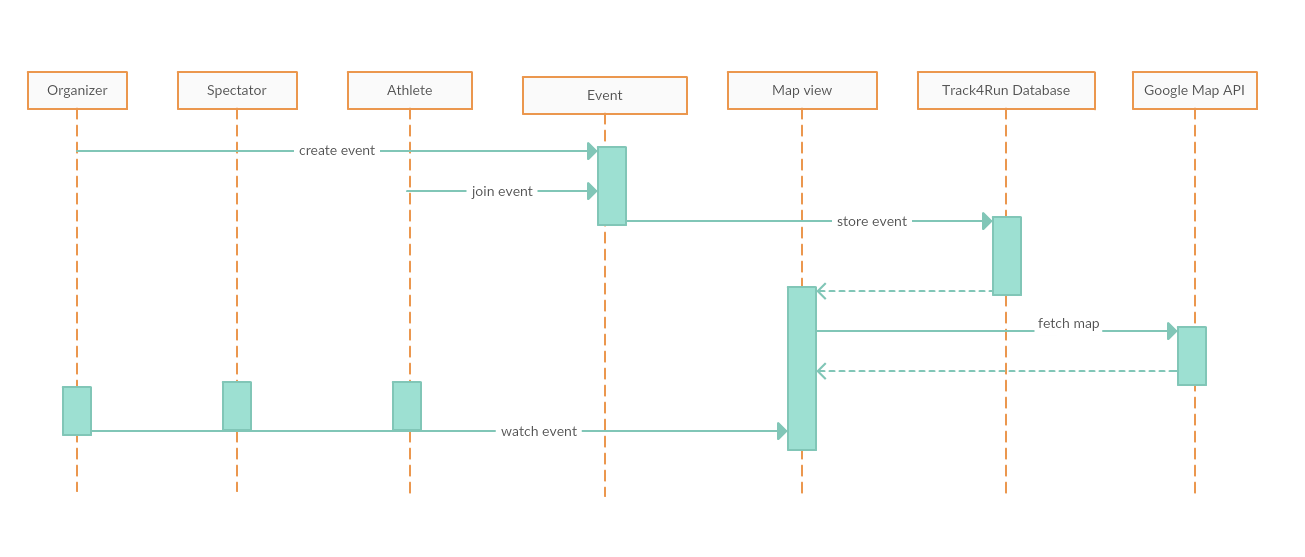
\includegraphics[width=\textwidth]{./DD_Diagrams/RuntimeAutomatedSOS.png}
      \caption{Sequence Diagram depicting runtime of AutomatedSOS Service}
        \label{TrackMe_r2}
	\end{center}
\end{figure}
\begin{figure}[H]
	\begin{center}
		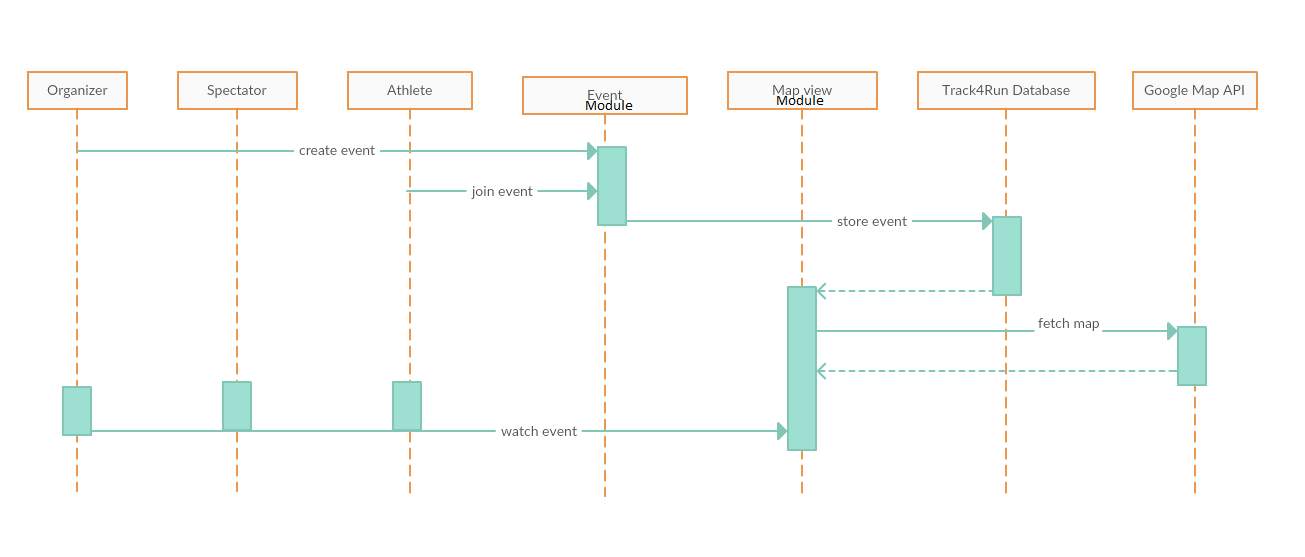
\includegraphics[width=\textwidth]{./DD_Diagrams/RuntimeTrack4Run.png}
      \caption{Sequence Diagram depicting runtime of Track4Run Service}
        \label{TrackMe_r3}
	\end{center}
\end{figure}